\section{Framwork}
\label{sec:framework}

\begin{figure*}[t]
  \centering
  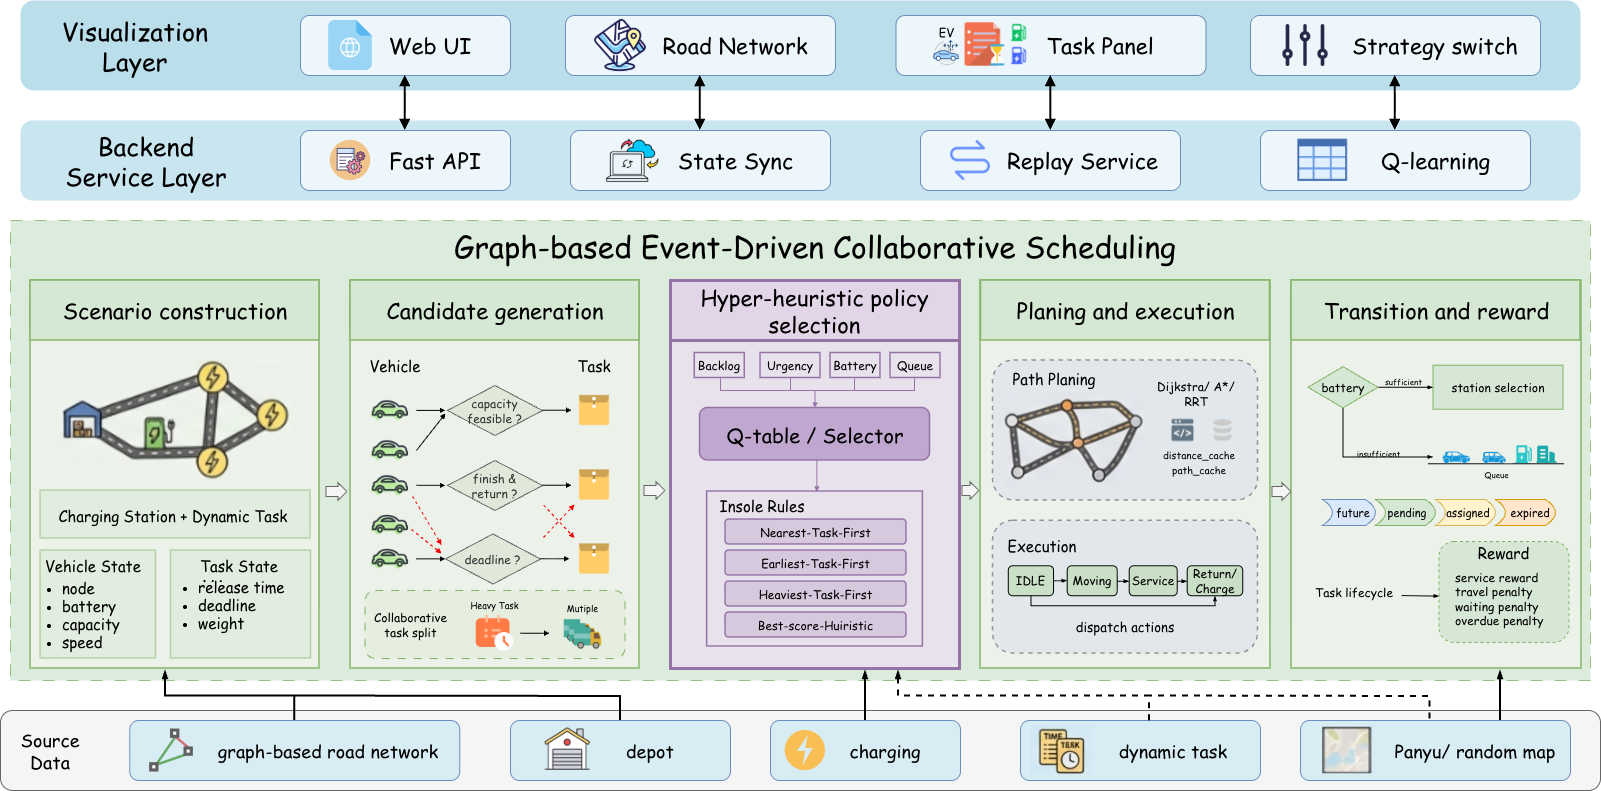
\includegraphics[width=\textwidth]{figure/framework.pdf}
  \caption{Overall framework of the dynamic collaborative scheduling system for new energy logistics fleets. The figure illustrates the relationships among the visualization frontend, backend service layer, simulation engine, scheduling strategies, path planning algorithms, and data resources.}
  \label{fig:framework_overview}
\end{figure*}

This paper designs a layered system architecture for the dynamic collaborative scheduling of new energy logistics fleets. Overall, the system can be divided into five core layers from bottom to top: the data resource layer, the algorithm layer, the simulation engine layer, the backend service layer, and the frontend visualization layer. Although each layer is relatively independent, they are connected through unified data interfaces and state transition logic to form a complete closed loop. This layered design has two main advantages. First, it decouples functions such as road modeling, path planning, scheduling decision-making, simulation execution, and interface presentation, thereby reducing overall system complexity. Second, it allows different path planning algorithms, scheduling strategies, and optimization methods to be flexibly replaced and compared within the same framework, which not only meets the implementation requirements of a course project but also supports further research and future extensions.

%-------------------------------------------------------------------------
\subsection{Data Layer}
The data resource layer provides a unified representation of the environment for the whole system and serves as the foundation for subsequent path planning, task scheduling, and state simulation. To satisfy the course requirement of using a graph structure for road representation and routing, this paper first models the urban delivery scenario as a weighted directed graph
\[
G=(V,E,W),
\]
where the node set \(V\) represents road intersections, depots, candidate task locations, and charging stations; the edge set \(E\subseteq V\times V\) represents road connectivity; and the weight function \(W:E\rightarrow \mathbb{R}^{+}\) describes the distance or travel cost of each edge. Based on this representation, the entire logistics environment can be mapped into a discrete graph space, which provides a computable foundation for shortest-path search, reachability analysis, and energy consumption evaluation.

In the implementation, the system denotes the depot as node \(v_d\in V\), the set of charging stations as
\[
S=\{s_1,s_2,\dots,s_m\}\subseteq V,
\]
and generates dynamic tasks from the candidate task node set \(V_T\subseteq V\). For any task \(\tau_i\), it can be represented as the following four-tuple:
\[
\tau_i=(r_i,\, v_i,\, w_i,\, d_i),
\]
where \(r_i\) is the release time of the task, \(v_i\in V_T\) is the task location, \(w_i\) is the cargo weight, and \(d_i\) is the deadline. This representation allows each task to include not only spatial information but also explicit time constraints, thereby supporting online scheduling decisions in dynamic arrival scenarios.

Furthermore, the data resource layer maintains the static parameter sets of vehicles and stations. For example, for vehicle \(k\), its state parameters can be defined as
\[
\mathbf{x}_k=(b_k^{\max},\, b_k,\, c_k,\, v_k^{\text{cur}},\, \eta_k),
\]
where \(b_k^{\max}\) and \(b_k\) denote the maximum battery level and current battery level, respectively; \(c_k\) is the load capacity limit; \(v_k^{\text{cur}}\) is the current node location; and \(\eta_k\) is the energy consumption per unit distance. For charging station \(s_j\), the system records attributes such as the number of chargers, queue length, and charging rate. In this way, the data resource layer provides not only the static topology of the road network but also a unified description of the parameters of tasks, vehicles, and charging facilities.



%-------------------------------------------------------------------------
\subsection{Algorithm Layer}
After the data resource layer completes the formal representation of the environment, the algorithm layer is further responsible for generating executable routing and scheduling decisions on the graph-based road network \(G=(V,E,W)\). In this paper, this layer is divided into two closely coupled basic modules: the path planning module and the task scheduling module.
\subsubsection{Path Planning}
For any vehicle \(k\) and target node \(v\in V\), the goal of the path planning module is to find a feasible path \(P_k(v_k^{\text{cur}}, v)\) on graph \(G\) from the current location \(v_k^{\text{cur}}\) to the target node \(v\). Let the total cost of a path \(P\) be
\[
C(P)=\sum_{e\in P} W(e),
\]
then the shortest path problem can be written as
\[
P_k^*(v_k^{\text{cur}}, v)=\arg\min_{P\in \mathcal{P}(v_k^{\text{cur}}, v)} C(P),
\]
where \(\mathcal{P}(v_k^{\text{cur}}, v)\) denotes the set of all feasible paths from \(v_k^{\text{cur}}\) to \(v\).

Based on this unified objective, the system implements three path planning baselines.
\begin{itemize}
  \item \textbf{Dijkstra:} A classic shortest-path algorithm for weighted graphs. It directly minimizes the total path cost \(C(P)\) and can stably return the global optimal path. Therefore, it is used as the standard shortest-path baseline in the system.
  \item \textbf{A*:} This method introduces a heuristic evaluation function \(h(u,v)\) on top of Dijkstra and uses
  \[
  f(n)=g(n)+h(n)
  \]
  as the search priority, where \(g(n)\) is the known accumulated cost from the start node to the current node \(n\), and \(h(n)\) is the heuristic estimated cost from \(n\) to the target node. This method maintains good search quality while reducing unnecessary node expansions, thereby improving the efficiency of each query.
  \item \textbf{RRT:} A sampling-based search method. It does not directly guarantee a strict shortest path in the graph sense, but explores a large state space through random tree expansion. This provides an interface for future research under more complex path planning settings.
\end{itemize}
In the new energy delivery scenario, path planning is not only used for travel from the current node to a task node, but also needs to support feasibility checking for returning to the depot after task completion and visiting a charging station when the battery is low. Therefore, for a task \(\tau_i=(r_i, v_i, w_i, d_i)\), the system not only computes \(C(P_k^*(v_k^{\text{cur}}, v_i))\), but also further evaluates whether the vehicle satisfies the basic energy consumption constraint. Let \(\eta_k\) denote the energy consumption per unit distance of vehicle \(k\). Then the energy consumption along path \(P\) can be approximately written as
\[
E_k(P)=\eta_k\, C(P).
\]
Only when the current battery level \(b_k\) is sufficient to support the planned trip is the path regarded as executable.

\subsubsection{Task Scheduling}
After feasible paths are obtained, the scheduling module further determines which task should be assigned to which vehicle. For the currently visible task set \(\mathcal{T}_t\) and the current state \(\mathbf{x}_k\) of vehicle \(k\), a baseline scheduling strategy essentially defines a priority score function \(\phi_k(\tau_i)\) over all candidate tasks and selects
\[
\tau_k^*=\arg\max_{\tau_i\in \mathcal{T}_t} \phi_k(\tau_i)
\]
as the task with the highest priority at the current time. The difference between different baselines lies in how the score function \(\phi_k(\tau_i)\) is defined.

\begin{itemize}
\item \textbf{Nearest-task-first strategy:} This strategy uses the minimum path cost as the main criterion. Its policy can be written as
\[
\tau_k^*=\arg\min_{\tau_i\in \mathcal{T}_t} C\bigl(P_k^*(v_k^{\text{cur}}, v_i)\bigr).
\]

\item \textbf{Maximum-weight-first strategy:} This strategy focuses on giving priority to high-load tasks. For a task \(\tau_i=(r_i,v_i,w_i,d_i)\), its policy can be written as
\[
\tau_k^*=\arg\max_{\tau_i\in \mathcal{T}_t,\, w_i\le c_k} w_i.
\]

\item \textbf{Earliest-deadline-first strategy:} This strategy takes task urgency as the main consideration, and can be expressed as
\[
\tau_k^*=\arg\min_{\tau_i\in \mathcal{T}_t} d_i.
\]
\end{itemize}

Beyond the above baselines, we further implement an online reinforcement learning policy selection module based on Q-learning, as well as an offline global optimization module based on MILP under full information. These two modules correspond to two different methodological paradigms: online decision-making based on interactive learning and offline solving based on exact optimization, as summarized in Algorithm~\ref{alg:qlearning_policy} and Algorithm~\ref{alg:offline_milp_planning}.

\begin{figure*}[t]
  \centering
  \refstepcounter{figure}\label{alg:qlearning_policy}
  \begin{minipage}{0.96\textwidth}
  \textbf{Algorithm \thefigure: Q-learning-based Policy Selection}
  \vspace{0.4em}
  \begin{algorithmic}[1]
  \Require training episodes \(M\), learning rate \(\alpha\), discount factor \(\gamma\), initial exploration rate \(\epsilon\), decay factor \(\rho\), discrete state space \(S\), action space \(A\)
  \Ensure learned Q-table \(Q\)
  \State Initialize \(Q(s,a)=0\), for all \((s,a)\in S\times A\)
  \For{episode \(=1\) to \(M\)}
      \State Reset the initial state \(s_0\)
      \While{the episode is not terminated}
          \State Generate a random number $k \in [0,1]$
          \State choose a random action \(a_t\) is random if $k<\epsilon$ else \(a_t=\arg\max_a Q(s_t,a)\)
          \State Execute action \(a_t\)
          \State Observe reward \(r_t\), next state \(s_{t+1}\), and the termination flag
          \State Update the Q-table:
          \State $Q(s_t,a_t)\leftarrow Q(s_t,a_t)+\alpha\bigl[r_t+\gamma \max_{a'}Q(s_{t+1},a')-Q(s_t,a_t)\bigr]$
          \State \(s_t \leftarrow s_{t+1}\)
      \EndWhile
      \State \(\epsilon \leftarrow \max(\epsilon_{\min}, \rho\cdot \epsilon)\)
  \EndFor
  \State \Return \(Q\)
  \end{algorithmic}
  \end{minipage}
\end{figure*}

\begin{figure*}[t]
  \centering
  \refstepcounter{figure}\label{alg:offline_milp_planning}
  \begin{minipage}{0.96\textwidth}
  \textbf{Algorithm \thefigure: Offline MILP-based Global Planning}
  \vspace{0.5em}
  Given the full-information task set \(\mathcal{T}\), vehicle set \(\mathcal{V}\), expanded node set \(\mathcal{N}\), and arc cost matrix \(C\), the offline planner solves the following mixed-integer linear program:
  \begin{equation}
  \min \sum_{v\in\mathcal{V}}\sum_{(i,j)\in\mathcal{A}} C_{ij}x_{vij}
  + \lambda_1 \sum_{v\in\mathcal{V}}\sum_{n\in\mathcal{T}} \mathrm{tardy}_{vn}
  + \lambda_2 T_{\max}.
  \end{equation}

  The optimization is subject to
  \begin{equation}
  \sum_{v\in\mathcal{V}} \mathrm{visit}_{vn}=1,
  \qquad \forall n\in\mathcal{T},
  \end{equation}
  \begin{equation}
  \sum_{j:(s,j)\in\mathcal{A}} x_{vsj}=\mathrm{use}_v,
  \qquad
  \sum_{i:(i,t)\in\mathcal{A}} x_{vit}=\mathrm{use}_v,
  \qquad \forall v\in\mathcal{V},
  \end{equation}
  \begin{equation}
  \sum_{i:(i,n)\in\mathcal{A}} x_{vin}
  =
  \sum_{j:(n,j)\in\mathcal{A}} x_{vnj}
  = \mathrm{visit}_{vn},
  \qquad \forall v\in\mathcal{V},\; n\in\mathcal{N}\setminus\{s,t\},
  \end{equation}
  \begin{equation}
  \mathrm{load}_{vj}
  \le
  \mathrm{load}_{vi}-w_j + M_{\ell}(1-x_{vij}),
  \qquad \forall v\in\mathcal{V},\; (i,j)\in\mathcal{A},
  \end{equation}
  \begin{equation}
  \mathrm{soc}_{vj}
  \le
  \mathrm{soc}_{vi}+\mathrm{chg}_{vi}-e_{vij}+M_b(1-x_{vij}),
  \qquad \forall v\in\mathcal{V},\; (i,j)\in\mathcal{A},
  \end{equation}
  \begin{equation}
  \mathrm{arr}_{vj}
  \ge
  \mathrm{arr}_{vi}+\mathrm{srv}_i+\mathrm{chgT}_{vi}+\tau_{ij}-M_t(1-x_{vij}),
  \qquad \forall v\in\mathcal{V},\; (i,j)\in\mathcal{A},
  \end{equation}
  \begin{equation}
  \mathrm{arr}_{vn}\ge r_n,
  \qquad
  \mathrm{tardy}_{vn}\ge \mathrm{arr}_{vn}-d_n,
  \qquad \forall v\in\mathcal{V},\; n\in\mathcal{T}.
  \end{equation}

  Solve the above MILP using Gurobi/CPLEX, decode the semantic route, and replay the resulting plan in the simulation engine for comparison.
  \end{minipage}
\end{figure*}
%-------------------------------------------------------------------------
\subsection{Simulation Layer}
The simulation engine layer is responsible for transforming the static environment defined in the data resource layer and the scheduling actions produced by the algorithm layer into an executable time-based process. It is the core component that enables dynamic closed-loop simulation in the whole system. Unlike methods that focus only on a single path query or a local dispatch decision, this layer explicitly models state variables that evolve over time, including task release, vehicle movement, battery consumption, charging queues, and task completion. In this way, the new energy logistics scheduling problem can be continuously solved and evaluated along a unified timeline.

In implementation, the system adopts a discrete-time update mechanism. Let the global environment state at time \(t\) be denoted by \(\mathcal{S}_t\), and let the joint action generated by the algorithm layer be denoted by \(\mathcal{A}_t\). Then, the simulation engine can be formalized as a state transition process:
\[
\mathcal{S}_{t+1} = \Phi(\mathcal{S}_t, \mathcal{A}_t),
\]
where \(\Phi(\cdot)\) denotes the environment transition operator jointly defined by task updates, vehicle movement, energy consumption updates, charging scheduling, and statistical recording. More specifically, at each time step, the system first adds newly released tasks into the pending-task set according to their release times and removes tasks that have already passed their deadlines. It then calls the scheduler to generate dispatch actions based on the current vehicle states and the candidate task set. After that, the system executes path movement and task service, while updating vehicle positions, remaining battery levels, load states, and task completion status. Finally, it processes charging-station events such as queuing, charger occupation, and battery replenishment, and synchronously refreshes system-level statistics.

The key role of this layer is to extend path planning and task scheduling from a \emph{static selection problem} to a \emph{dynamic evolution problem under resource constraints}. For example, when vehicle \(k\) travels along path \(P\), its battery level decreases continuously according to the energy consumption model defined earlier, namely \(E_k(P)=\eta_k C(P)\). When \(b_k\) is no longer sufficient to support the planned trip, the simulation engine triggers charging-station selection and queueing logic, and updates the waiting state under limited station capacity. Similarly, for dynamically released tasks, the simulation engine determines not only when a task enters the assignable set, but also whether it becomes a penalty item because of deadline violation. As a result, metrics such as task reward, vehicle utilization, path length, and charging load can all be computed consistently within a unified simulation framework.



%-------------------------------------------------------------------------
\subsection{Frontend and Backend}

The frontend layer and the backend layer do not directly participate in path planning or scheduling optimization itself. Instead, they are responsible for organizing the states, events, and statistical results inside the simulation engine into external representations that are accessible, replayable, and analyzable. In this way, the whole system is equipped with a complete experimental loop and interactive capability.

In implementation, the backend is responsible for unified state packaging and service exposure. The system uses FastAPI and WebSocket to establish a persistent communication channel, and projects the environment state \(\mathcal{S}_t\) at time \(t\) into frontend-consumable data objects, such as vehicle positions, task states, charging-station load, accumulated score, and event logs. At the same time, the backend also receives control commands from external users and converts them into invocation requests for the simulation process or algorithm modules. In addition to standard controls such as start, pause, resume, and stop, this layer also provides unified interfaces for Q-learning training and inference, offline MILP solving, and result export, so that the experimental process can be scheduled and reused within the same service framework. In other words, this layer essentially provides a mapping
\[
\Psi: \mathcal{S}_t \mapsto \mathcal{O}_t,
\]
where \(\mathcal{O}_t\) denotes the structured observation result for external interfaces, thereby converting complex low-level states into standardized service outputs.

On this basis, the frontend visualization module further transforms \(\mathcal{O}_t\) into graphical expressions that can be easily understood by users. Specifically, the interface continuously displays the spatial distribution of the road network, depots, task nodes, charging stations, and vehicles, while synchronously updating key indicators such as task completion status, vehicle utilization, path cost, charging queue length, and system score. More importantly, this layer does not only serve as a static display component. It also provides a unified interaction entry for policy switching, offline replay, training triggering, and result comparison. As a result, the multi-source information originally scattered across simulation logs, scheduling outputs, and statistical results is reorganized into a visual workflow for analysis and presentation.

